\section{User Evaluation}\label{sec-user-evaluation}

User testing and evaluation \replace{is}{will be} carried out throughout the project and 
\replace{on several levels}{with regard to several aspects}:
\begin{itemize}
\item Components
\item Platform Integration
\item Prototypes
\item Usability 
\end{itemize}


\subsection{User Testing at the Component Level}

%\UG{I'd skip the introductory text here and start straight with ASR.}

%Component testing focuses on the different technologies and components, e.g. ASR, MT, summarisation, clustering, semantic analysis. As mentioned before, evaluation timing depends on the availability and new releases of the components.

Evaluation methods differ per component, due to the nature of the activity, and per partner, depending on the use of the tool. 


The following technologies/components are covered in the project:
\begin{itemize}
\item ASR: Speech recognition
\item Meta: Metadata extraction from broadcast media
\item MT: Machine translation
\item CT: Streaming implementation of Storyline Clustering and Topic detection 
\item ETL: Entity Tagging \& Linking 
\item KB: Knowledge Base Construction
\item FC: Forecasting and Fact Checking
\item SP: Story-level semantic parsing 
\item SH: Story highlight generation/summarisation
\item SS: Story-level sentiment analysis
\end{itemize}


\subsubsection{\ins{Automatic Speech Recognition  (}ASR\ins{)}}

%\UG{The use of DW vs Deutsche Welle is inconsistent within the document. I'd choose one and stick with it. Otherwise the document reads like patchwork from different authors. - done}

Deutsche Welle test users will test the ASR in different ways: (1) trialling the functionality of the component through request and visual assessment of automated transcription in the platform; (2) manual quality control, i.e., by comparing some of the \SUMMA automated transcript output to the original editorial scripts.  Comparison will be done in first instance with a difference spotting tool, e.g. Diffchecker (https://www.diffchecker.com/diff), and subsequently humanly assessed. This will be done for specifically selected content assets. A second comparison method that will be used is comparing the usability of the output to that of other ASR tools available to Deutsche Welle for the same language. User assessment of ASR output quality focuses on fidelity (correctness, reliability of the information, including names entities), readability of the output (including punctuation) and overall usability by reading the automated transcripts in the original language. Assessment of ASR output will take different types of content (as to noisiness) into account.

%\subsubsection[fragile]{\ins{Machine Translation (}MT\ins{)}}l\label{sec:validation-mt}

\subsubsection{\ins{Machine Translation (}MT\ins{)}}
\label{sec:validation-mt}

\cut{n Task 7.2 we indicated early user evaluation of individual features and functions of the \SUMMA platform, and this includes evaluation of MT performance.} The main us\cut{ag}e of MT in \SUMMA is to assist journalists in monitoring the media in some vernacular, like Russian or Spanish. MT here can help them either if they are not an expert in all the languages that they want to monitor (ingestion), or it might help them to actually produce texts in English, with subsequent postediting. MT is also helpful for source monitoring, where rough streams of information are passed on to customers. 

One \replace{evaluation method is}{approach to evaluating the usefulness of MT for end users is the use of} gap filling tests. Gap filling measures the level of comprehension of the translated document. Document-level comprehension tasks are usually measured by comprehension questions. Comprehension questions are very time consuming to create, and result in a low coverage of the documents content. It is also laborious to evaluate the results of comprehension questions. Gap filling is seen as a more efficient and reliable way of extracting document-level comprehension scores. The gap filling task \replace{comprises of}{starts with} an evaluator reading a machine-translated article. Then they are presented with one or more human translated sentences where important content words are removed. They are asked to fill in the gaps. The quality of the machine translation is measured by the evaluator's success in filling in the gaps correctly, and how long it takes them. 
We will run a gap filling evaluation in \replace{y}{Y}ear 2 of the project. We will test German, Arabic, Farsi, Russian and Ukrainian translation models, and we will test broadcast media and newswire data sources. We will also provide information specifically about Named Entities and numbers. This will allow us to provide a quantitative measure for how much of the key information in an article is translated in a way that humans can understand. These exercises will require test users who are fluent in the target language (e.g. native speakers). Specific languages will be tested as and when the relevant components have been released.  
 
\begin{itemize}
\item The BBC will participate in gap filling tests in collaboration with the MT team. This includes evaluation for  Arabic and Russian in Y2 (Q1 or Q2); and for Farsi and Ukrainian in Y2 (Q3). Depending on the readiness level of these components, the gap filling exercises might take place nearer the end of Y2. These exercises will require test users who are fluent in the target language (e.g. native speakers).

\item Deutsche Welle will test the MT tool in different ways: (1) taking part in gap filling tests, as requested by technology partners, e.g. for German. (2) trialling the functionality of the component through visual assessment of machine translated output in the platform; (3) quality control through comparison, i.e., by comparing some of the \SUMMA automated MT output to existing (manually produced) Deutsche Welle translations. Comparison will be done in first instance with a difference spotting tool, e.g. Diffchecker (https://www.diffchecker.com/diff), and subsequently humanly assessed. This will be done for specifically selected content assets. A second comparison method that will be used is comparing the usability of the output to that of other MT tools available to Deutsche Welle for the same language pairs. User assessment of MT output quality focuses on fidelity (correctness, reliability of the information) and usability and intelligibility (readability of the translation) by reading the translations.
\end{itemize}

\subsubsection{Clustering and Topic Labelling (CT)}\label{sec:validation-clustering}

Evaluation of the \SUMMA clustering technology for monitoring purposes will be done by the user partners, who have access to the separate clustering demo developed by Priberam. User feedback on this component is provided as of the first release \ins{at the} end of \replace{y}{Y}ear 1. 
The selection, formulation and usefulness of the clustered storylines are assessed based on the output in the clustering component. Feedback is provided directly to the developing partner and recorded in the \SUMMA wiki. Ideally, the user feedback will evaluate the following two components of the system in separate: (i) the visualisation interface; (ii) the generated storylines. The generated storylines would be evaluated according to (a) their granularity (if they are too fine or too coarse), (b) their quality (if the news documents in the same storyline are indeed related) and (c) their usefulness to each user persona.

Topic labels or keywords for individual stories can be used in several ways for the end-user applications, depending on the use case.  For external monitoring, keywords can be used as filters to detect topics of interest, in which case the component can be evaluated by estimating the number of false positives and false negatives.  However, our approach to multilingual representation learning and cross-language transfer is more specifically dedicated to a fully-multilingual internal monitoring use case, where it is able to output keywords in any language for inputs in any language.  Therefore, the component is able to indicate, to each language-specific service, what topics are active in other languages and might need fuller treatment in a given language.  Such a scenario should serve as the basis for user-oriented evaluation, e.g.\ by observing whether the system helps users to avoid gaps in news topics more easily than without it. The BBC will carry out user evaluation sessions for this component.


\subsubsection{Entity Tagging \& Linking (ETL)}\label{sec:validation-etl}

The contribution of the Entity Tagging \& Linking (ETL) module to the \SUMMA platform is twofold. On the one hand, the text visualised in the explorer tab will be enriched with mentions marked with entity types and with entries in the knowledge base. On the other hand, the schemes summarising the trending entities of a query will be computed based on a collection of news that were marked with entities’ information.

Regarding user evaluation, we would like to have qualitative feedback (for example, a qualitative number from 1 to 5), from each user persona, on both the usefulness and quality of the ETL module. In particular, the user feedback would evaluate the following components of the module in separate: (1) if the spans of the mentions are correctly detected; (2) if the entity types are correctly assigned; (3) if the mentions were correctly disambiguated with entries in the knowledge base (4) and if there are many undetected mentions. The BBC will carry out user evaluation sessions for this component.

\subsubsection{Knowledge Base Construction (KB)}

The success of our knowledge base construction efforts should ultimately be judged in terms of its utility to end users. This utility might take two forms. The first takes the knowledge base as a stand alone entity, with its usefulness being related to the accuracy and coverage of the facts it contains. In this case, evaluation would be similar to the TAC-KBP task mentioned above. The second views the underlying documents as the objects of interest to the users, and the extracted relations as merely an aid to understanding their contents. In this case, evaluation could be more like that for summarisation.

Ultimately, both aspects are probably important. One possible approach to user evaluation would be to have one set of users identify queries (e.g. ``Who is the finance minister of Kenya?'') of interest for a document collection, then evaluate the ability of another set of users to find the correct answers and source documents from the extracted knowledge base.

\subsubsection{Fact Checking (FC)}\label{sec:validation-fact-checking}

Given the nature of fact-checking it is useful to have a user evaluation. A mock up including fact checking was presented in the Project Meeting in Lisbon in November 2016. The truth assessments by the system should be integrated via an appropriate interface which will allow the user to give feedback on the following aspects:
\begin{itemize}
\item correctness of the truth assessment
\item correctness of the provenance, since a system can return the correct assessment for the wrong reasons
\item usefulness of the system, since the assessment might be wrong, but the provenance information can still be useful
DW will participate in this exercise.
\end{itemize}

\subsubsection{Story-level semantic parsing (SP)}\label{sec:validation-semantic-parsing}

User evaluation might be used here in two ways: (1) creating a small hand-annotated corpora for AMR for German and Spanish that we could evaluate the parser with. This will be made possible, we hope, by getting access to the AMR GUI tool that is available for annotation in English (developed at ISI, \url{http://www.isi.edu/}); (2) evaluating the quality of AMRs output by our parsers (for all languages, English, German and Spanish) similar to the way it is done with machine translation in the yearly MT competition at Edinburgh. This will be done when all parsers mature significantly, to avoid this costly process being repeated.

Creating the small hand-annotated corpora will be led by \cut{a student (}Marco Damonte\cut{)}, and we \replace{hope}{expect} to complete this process by the end of the summer 2017. Manual evaluation of the quality of AMR parser outputs will be done subsequently.

We also note that the SemEval shared task this year includes a human evaluation component.


\subsubsection{Summarisation and Sentiment Analysis (SH - SS)}\label{sec:validation-summarisation}

Evaluation of topical reliability, usefulness, readability of summaries will be done by the two user partners by assessing the quality and usefulness of the output in the \SUMMA platform. Specific feedback on this component will be provided directly to the developing partner and recorded in the \SUMMA wiki. 

General feedback is expected about the utility of the system in the tasks each partner judges most important. This feedback may be provided per screen view or in a global way. The feedback may be given in the form of a questionnaire or a simple judgement if it is satisfactory or not.

The possible topics for a course level evaluation of the summaries are:  (a) the utility of their informativeness level (if they are too fine or too coarse in given the facts happened in the cluster), (b) their quality (if the summaries are well presented and understandable) and (c) their usefulness to each user persona.

The sentiment analysis may follow the same approach, with the possible topics for a course level evaluation being (a) their accuracy level (if they correspond to what is reported), and (b) their usefulness to each user persona.
The BBC will carry out user evaluation sessions for this component.


\subsection{Integrated Platform Testing}

%\UG{Shouldn't this section go into Section \ref{sec:verification}? It seems to be more about technical testing than user testing. - done}


\subsubsection{Platform Testing}

Most evaluation will be done by LETA on the integrated platform, as described in section 3.3. In parallel to the technical functionality evaluation, the semantic evaluation of the integrated NLP system will be performed routinely to ensure the semantically correct data flow of data through the \SUMMA Platform. This part of debugging and evaluation will be based on rigorous evaluation of the video, audio and textual inputs and outputs through the support for experiment reproducibility to enable pinpointing of the seldom occurring semantic errors.

Users, for instance Deutsche Welle, will evaluate the platform upon request in function of the output produced by the platform, regardless of the UI. It will also evaluate the output in the integrated platform compared to the output of the separate components. This will evaluate, for instance, if any useful details or functionalities from the components are lost in the integrated platform. On the other hand, it also evaluates the added value of the technologies/components through the combination of the technologies in the integrated platform. For example, the summarisation tool has its own platform and the use of that separate platform will be compared to its use in the integrated platform.

\subsubsection{Scalability Testing}

For the BBC this includes available and relevant media streams and content sources. Initially, for up to 36 streams the level of monitoring will measure stability of the architecture and the increase of number of channels monitored per journalist. The available sources will be transcribed and translated to English as well as clustered into storylines. We will be testing 250–400 media 
streams to observe crucial patterns in the large data sets. These numbers of streams will be appropriate for regional analytics.

For the Deutsche Welle internal monitoring use case this means all recently produced data published in those languages covered by the project, i.e. a daily increase of some 12h of audiovisual data, plus text items.

\subsection{Prototype Testing}

This type of testing is part of iterative agile prototyping. Functionality testing begins in \replace{y}{Y}ear 1, as soon as the first prototype is available. Testing is done regularly and upon a new release or update of the platform or at the integrator’s request. It is repetitive, regular, with a fast feedback cycle, and will follow user test scripts. A regular feedback schema will be established to ensure regularity of testing.

The objective at this stage is to answer questions such as: “Does it work? Does it do what I expect it to do?” etc. We also want to determine here whether there is an efficient flow between the different functions, e.g. ASR, MT, clustering, search features, user management, etc.

All technical elements of the user interface and its associated user functionalities will be tested. The design will emerge from
a better understanding of the architecture, as well as potential failure points and the business impact of any of these. The
lab test and field test protocols for data streams as well as the scalability of streams will evolve with the prototyping
progress. The objective of functionality testing is to see how the system responds according to the design specifications collated in WP1.

Weekly feedback meetings will communicate functional test results to the business analyst and software developers team. They will be able to discuss and analyse user feedback such as reported bugs and snags or requested enhancements. JIRA will be the primary tool for the logging and tracking of functionality test feedback, which will contribute to the prototype design. It will benefit the agile prototyping team, user partners and technical partners.

All features and functionalities identified in WP1 will be tested systematically as and when they are released to the platform environment. They form part of the backlog and will be developed in sprints. As specified in the user requirement analysis, functional testing includes:

\begin{itemize}
\item monitor sources
\item manage feeds
\item manage social media
\item play video and audio
\item display text sources
\item create transcription in original language
\item create translation into English
\item generate trend analysis
\item generate breaking news alerts
\item generate news story
\item generate storyline
\item detect names entities
\item create summaries
\item cluster stories and storylines
\item perform a search
\item manage user profile and preferences
\item teaser
\item UI performance
\end{itemize}

\subsubsection{Feedback Flow}
The flowchart \replace{below}{in Fig.~\ref{fig:tracking_user_feedback}} outlines the process for providing and tracking user feedback as part of the agile prototyping. The feedback from the tester is analysed by the project manager, then discussed with other project managers at consortium level, and finally passed on to the developer for action in case of a defect or requested enhancement. 
%\UG{The figure has small print and is therefore hard to read. Consider putting it in landscape mode on a separate page}



\begin{figure}[ht]
    \centering
    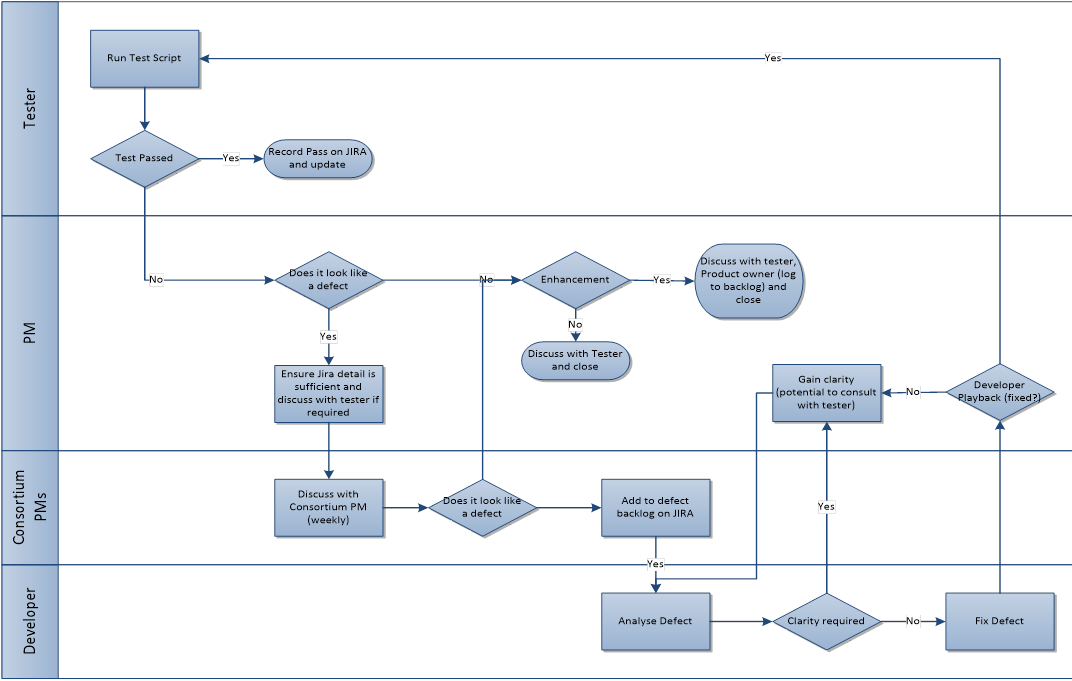
\includegraphics[width=1\textwidth,angle=270]{./images/test_script_JIRA.png}
    \caption{Tracking User Feedback Process}
    \label{fig:tracking_user_feedback}
\end{figure}



\subsection{Usability Evaluation}

Usability is understood as the extent to which a product can be used by specified users to achieve specified goals with effectiveness, efficiency, and satisfaction in a specified context of use. 

This is at the use-case level and will be an iterative process throughout the project. The demonstrators will be implemented on top of the integrated \SUMMA platform, and can be customised for the different user partners. Initially testing will happen on the common prototype, and later on enhanced with the specific customised dashboards. 

This evaluation involves end users in a near-life environment, in lab and field trials. It will engage professional users, such as monitors, editors, journalists, to test the use case in a (simulated) working environment. The question here is: ``Is the \SUMMA platform fit for purpose?''  The user evaluation is primarily aimed at testing usability to find out whether our intended users are happy with what \SUMMA can do for them. 

Usability tests are carried out with an initially small test user group. It will gradually be expanded and additional test users from the target group are involved at both user partner sites.

User feedback will be collected digitally, for instance by means of an online form, with automated analysis and visualisation. This will gather feedback on ease of use, usefulness and user satisfaction. In addition to regular feedback cycles, special events such as user days, workshops, etc. will be organised to introduce the system to other user groups. Feedback is provided directly to the technical partner concerned or the entire consortium, fed into the JIRA system, and recorded in the wiki.

Since Deutsche Welle and BBC have different use cases and target groups, the evaluation at this level will be carried out separately, and the feedback mechanism will be coordinated. Deutsche Welle will primarily engage editorial teams at different levels; the BBC will involve monitoring journalists and other editorial staff. Each user partner will be responsible for preparing the test material for their test users, and for scheduling and carrying out their test sessions.

\subsubsection{External Monitoring Use Case}
Monitoring Journalists will in the main be using \SUMMA as a tool to point it to important events, entities and trends in the ingested media occurrences. Perfection in the ASR, machine translation and summarisation results will not be the focus in this particular use case. Results in spotless grammar will not be required. So, for example, in the majority of cases, the inaccurate rendering of a plural as a singular or vice versa will not affect the usefulness of the system. 

More important, however, is accuracy of substance. The regular omission (or spurious addition) of ‘not’ would be a fairly serious problem. Therefore, the user evaluation of Use Case 1 will be focusing more on the output quality of the overall platform rather than comparing machine translation with human translation or ASR with human transcription.
\medskip

\textbf{User Evaluation Approach:} 

\textbf{Phase 1:} usability testing during the development of the initial prototype (Lab Tests)

1. Definition of key tasks which the users want to complete with the \SUMMA platform. 

2. Usability sessions: User observations and structured one-to-one interviews. A small number of test users will use the platform during scheduled sessions outside their operational hours for short periods of time. A member of the project team will observe the user and ask the user specific questions about the usability of the platform (e.g. are the key tasks easy to complete with this platforms?) as well as the quality of the output (e.g. accuracy of proper nouns, omission of essential words, relevance of story clustering etc.). Test users will have experience in media monitoring in the context of world news and will be fluent in one of the business critical languages: Arabic, Russian, Farsi, Ukrainian. They will trial all of the personae identified for Use Case 1. 
\medskip

The focus on particular languages depends on the component release. The BBC will be working closely with the relevant technical partners to schedule the usability sessions accordingly.
\medskip

\textbf{Phase 2:} usability testing during the development of the improved prototype (Field Tests)
\smallskip

This test user group will include operational staff who will be asked to include the \SUMMA platform in their live operational workflow for a set period. Members of this test group will be fluent in one of the business critical languages (Arabic, Russian, Farsi, Ukrainian), and will be experts on the  media landscape of the relevant geographical region.


\smallskip

1. Usage analytics will be incorporated to capture actual usage statistics. This will add automated quantitative feedback to the qualitative focus of these tests (e.g. how long did it take the user to complete their task).

2. Short questionnaires will be filled in by the test users. Structured one-to-one interviews might be carried out as well as user observations with a select number of users. 

3. Optionally, as an alternative to user observations and structured interviews, a Diary Study can be carried out: test users will be asked to keep a journal to capture their experience with the platform. The main focus of the diary analysis will be the same as in phase 1: usability of the platform and quality of the output. The journals can be captured in the form of a daily prompt by email, for example at the end of the journalists' shift, while their experience with the platform is still fresh in their memory.
\medskip

User participation in Phase 2 very much depends on staff availability and changing business requirements at the time. The nature of BBC Monitoring operations is defined by world news events to which they need to respond at very short notice. Therefore, the user evaluation plan needs to be flexible enough to fit around the live operations with as little interference as possible.
\medskip


\textbf{Technology Testing:}
The components for 
Machine Translation (Sec.~\ref{sec:validation-mt}), 
Clustering and Topic Labelling (Sec.~\ref{sec:validation-clustering}), 
Entity Tagging and Linking (Sec.~\ref{sec:validation-etl}), and 
Summarisation and Sentiment Analysis (Sec.~\ref{sec:validation-summarisation}) 
will also be evaluated by BBC test users. The focus will be on qualitative evaluation. Its purpose is to support the research efforts of the technical partners involved in WP3 and WP5. Machine Translation will be evaluated through gap filling exercises in collaboration with the MT team. The evaluation of WP 5 technologies will be carried out during three 'checkpoint' evaluation sessions which are scheduled for Year 2 and Year 3; the sessions will be carried out in the lab environment and will last for approximately 4 hours each. The test language will be English. While test users carry out key tasks (see above, Phase 1) they are asked to judge the quality of clustering, topic labelling, summarisation, sentiment analysis and entity tagging. This will either be part of short questionnaires or structured one-to-one interviews as described above. A simple rating system will be used (e.g. rate the quality on a scale from 1 to 5) which can be integrated into the user interface for test purposes. Field tests are desirable, but very much depend on staff availability at the time.



\subsubsection{Internal Monitoring Use Case}

Deutsche Welle will test the tool in different ways throughout the project. End users will be involved on a semi-continuous basis. The released  platform will be introduced to the different language departments with the request to use it on a regular basis and to provide feedback through the online feedback system integrated in the platform (in the form of like/dislike buttons and comment fields). This includes several stakeholders, such as journalists, editors, heads of region and language groups covering the different \SUMMA languages. The users will focus on Deutsche Welle content provided to \SUMMA via the Deutsche Welle API. DW \SUMMA project managers will be in charge of coordinating evaluation sessions at Deutsche Welle. 

In addition, specialists from Deutsche Welle’s Innovation Division contribute by focusing on specific innovative aspects, applications and visualisations, providing a different point of view, and will form focus test groups for consistent testing.

Evaluation in \replace{y}{Y}ear 2 will be on the V2 prototype using the LETA Integrated Platform. Different functions will be assessed in terms of user expectations, quality and format of output, ease of use.  

This includes, for instance, feedback on the following \SUMMA output that can help the journalist/editor in his journalistic tasks:

\begin{itemize}
\item preview and quality of video
\item usefulness of the teaser
\item usefulness of the summary
\item overview through stories and storylines
\item selection of feeds
\item completeness and accuracy of named entities
\item quality of transcript in original language
\item quality of transcript in English
\item usefulness of keywords and tagging
\item monitoring enhancement through alerts
\item search facility
\item user management, preference setting
\item possibility to train the system
\item overall UI issues
\end{itemize}

In addition to such continuous feedback method, Deutsche Welle will also organise user days, workshops, etc. to engage a larger user group, both internally and within the DW network. 

There will be minimally three set user evaluation sessions spread out over years 2 and 3. For such end-user sessions, user instructions, guidelines and pre-set task descriptions will be prepared to ensure smooth and clear user trials. Screencasts will be made, serving as an online demo of the tool. In a typical session, the user will be presented with the \SUMMA tool, containing a variety of functionalities, depending on the stage of development, and then asked to perform a series of pre-set tasks. A certain amount of autonomy will also be accorded to the user so that s/he can “play” with the tool and be creative in their way of using the system.

Feedback will be gathered in different ways, including:
\begin{itemize}
\item personal interviews: collecting personalised feedback during one-on-one sessions
\item questionnaires: these will be produced and made available online and are used to gather consistent user feedback – and the output can easily be analysed and visualised 
\item direct feedback on contents appearing on screen through feedback buttons and user behaviour analysis:
\begin{itemize}
\item Like/Dislike buttons
\item Keep for later button
\item Never show again button 
\end{itemize}
\end{itemize}

\begin{figure}[ht]
    \centering
    
\includegraphics[width=0.2\textwidth]{./images/like_dislike.jpg}
    \caption{Like-Dislike Buttons}
    \label{fig:like-dislike}
\end{figure}


\subsubsection{Data Journalism Use Case}
The third Use Case (Data Journalism) will be developed in the course of the project and evaluation will be tailored to that use case. Some aspects will be similar to or in parallel with the evaluation of the monitoring use cases, but it will not be limited to that. Data journalists are likely to be using the \SUMMA platform with a different focus than monitoring journalists. Key tasks which they need to complete might be different from those established in \replace{u}{U}se \replace{c}{C}ases 1 and 2, and need to be identified first. Therefore, it is sensible to develop the usability test plans accordingly. The user requirements for and the design of the third prototype will determine the evaluation techniques of use case 3.

\subsubsection{Schedule of User Testing}

User testing scheduling obviously depends on the availability and release of the prototypes. Moreover, agile prototype development will be applied in \SUMMA and therefore assumes a regular feedback cycle. Thus, as explained in the sections above, user evaluation takes place throughout the project.  Three `checkpoint’ evaluation sessions of selected technologies are planned by the two broadcasters, in line with the milestones and depending on prototype release, e.g., middle of Y2, early Y3 and at the end of Y3 (project end).\SW{I’ve refined the ‘checkpoint’ sessions bit because it only applies to Priberam’s technologies (for the BBC anyway).}



 


